\documentclass[12pt]{report}
\usepackage[utf8]{inputenc}
\usepackage[T1]{fontenc}
\usepackage[francais]{babel}
\usepackage{titlesec}
\usepackage{amsmath}
\usepackage{amssymb}
\usepackage{layout}
\usepackage{pdflscape}
\usepackage{graphicx}
\usepackage[top=2cm, bottom=2cm, left= 2.5cm, right=2.5cm]{geometry}

\title{Projet Advance Wars}
\date{\today}
\author{Pierre MARIET - Joanna XANH\\
3\up{ème} année, Option Informatique et Systèmes}
\begin{document}

\begin{figure}

\includegraphics[width=60mm, height=65mm]{logoENSEA.png}
\end{figure}

\maketitle
\thispagestyle{empty}
\newpage

\tableofcontents
\newpage

\chapter{Présentation générale}
    \section{Archétype}
    \paragraph{}Le projet est de recréer le jeu Advance Wars\textsc{\texttrademark} développé par Intelligent Systems\up{\textregistered} pour la Game Boy Advance\textsc{\texttrademark} de Nintendo\up{\textregistered}.\newline
    Le jeu est en tour par tour, sur une carte découpée en cases. Le but du jeu est de capturer le Quartier Général adverse. Il est aussi possible de gagner par forfait. Les cartes pourront être crées à partir d'un fichier texte.
    \section{Règles du jeu}
    \subsection{Description des unités}
    \paragraph{}Sur une carte composée de différents terrains et séparée en cases s'affrontent 2 armées. Les terrains augmentent ou non la défense de l'unité qui se trouve dessus. Ces armées sont composées de différentes unités qui ont chacune des spécificités qui varient :
    \begin{itemize}
        \item Les unités aériennes peuvent se déplacer n'importe où sur la carte. Les unités de transport aérien ont une capacité de 1 et ne peuvent débarquer en mer ou en montagne.
        \item Les unités navales ne peuvent se déplacer qu'en mer, pas dans les rivières. Les unités de transport naval peuvent débarquer uniquement sur une plage ou dans un port.
        \item Les unités d'infanterie et bazookas peuvent se déplacer sur tous les sols et traverser les rivières.
        \item Les unités terrestres motorisées ne peuvent franchir les montagnes.
    \end{itemize}
    \subsection{Les généraux et leurs pouvoirs}
    \paragraph{}Chaque armée est dirigée par un général possédant un pouvoir qui donne un avantage à son armée ou un inconvénient à l'ennemi. Ce pouvoir dure un tour (sauf dans pour le Blizzard) et se recharge sur plusieurs tours. Le général donne en plus un avantage moindre, ou non, mais en rapport avec son pouvoir et qui dure toute la partie.
    
    
        \paragraph{Réparation}Redonne 2 points de vie à toutes les unités alliées. Aucune autre spécificité en dehors du pouvoir.
        Les statistiques de ce général représentent les statistiques moyennes.
        
        \paragraph{Blizzard}Provoque une tempête de neige qui dure deux tours et qui diminue l'amplitude de déplacement des unités adverses.
        Aucune autre spécificité en dehors du pouvoir.
        
        \paragraph{Marche forcée}L'infanterie peut se déplacer d'une case en plus et les bazookas ont une force de frappe augmentée de 50\%.
        Par défaut, l'infanterie et les bazookas ont un bonus de force de frappe de 20\% et de 10\% de défense contre les unités d'infanterie adverse. Une unité qui capture un bâtiment a vitesse de capture de 150\% de ses points de vie.
        La puissance de frappe des autres unités de tir direct est en revanche moins élevée que la moyenne. Les unités de transports peuvent se déplacer d'une case en plus par rapport à la moyenne.
        
        \paragraph{Puissance Max}Les chars d'assaut voient leur puissance de frappe augmenter de 40\%, leur défense augmente de 1 point et leur amplitude de déplacement augmente de 1 case.
        Par défaut, les chars d'assaut ont une puissance de frappe 50\% plus élevée que la moyenne.
        
        \paragraph{Embuscade}Les unités de tir indirect voient leur portée augmenter de 1 et leur force de frappe augmenter de 50\%.
        Par défaut, la portée des unités de tir indirect est augmentée de 1 case. Les unités de tir direct ont une force de frappe diminuée de 20\%.
        
        \paragraph{Frappe éclair}Les unités aériennes peuvent se déplacer une nouvelle fois pendant le tour.
        Par défaut, la force de frappe des unités aériennes est 15\% plus élevée que la moyenne Les forces navales ont une force de frappe réduite de 20\% par rapport à la moyenne.
        
        \begin{figure}[h]
    \begin{center}
    
\includegraphics{advance_wars_sprites_andy.png}
    
\includegraphics{advance_wars_sprites_olaf.png}
    
\includegraphics{advance_wars_sprites_sami.png}
    
\includegraphics{advance_wars_sprites_max.png}
    
\includegraphics{advance_wars_sprites_eagle.png}
    
\includegraphics{advance_wars_sprites_gritt.png}
    \end{center}
    \caption{Sprites des généraux}
    \end{figure}
    
    \section{Ressources}
    \paragraph{}Les ressources graphiques utilisées sont celles du jeu d'origine. Néanmoins, en considérant le temps de développement des autres paramètres du jeu, seuls la carte, les unités sur celle ci ainsi que les animations de capture seront affichées.
    
    \begin{figure}[h]
    \begin{center}
    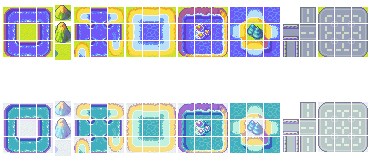
\includegraphics{advance_wars_sprites_map_tiles.png}
    \end{center}
    \caption{Sprites pour les tuiles de la carte}
    \end{figure}
    
    \begin{figure}[h]
    \begin{center}
    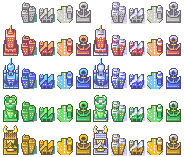
\includegraphics{advance_wars_sprites_cities.png}
    \end{center}
    \caption{Sprites des différents batiments de la carte}
    \end{figure}
    
    \begin{figure}[h]
    \begin{center}
    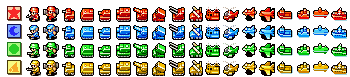
\includegraphics{advance_wars_sprites_units.png}
    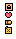
\includegraphics[scale=1.8]{advance_wars_sprites_units_info.png}
    \end{center}
    \caption{Sprites des unités ainsi que les informations de statut}
    \end{figure}
    
    \begin{figure}[h]
    \begin{center}
    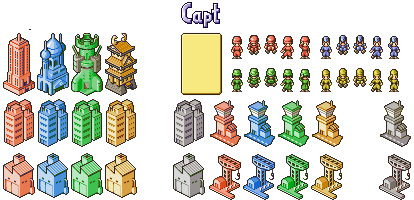
\includegraphics{advance_wars_sprites_capture.png}
    \end{center}
    \caption{Animations de capture}
    \end{figure}
    
    \begin{figure}[h]
    \begin{center}
    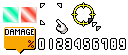
\includegraphics{advance_wars_sprites_damages.png}
    \end{center}
    \caption{Sprites des fenêtres d'attaque}
    \end{figure}
    
\chapter{Description et conception des états}

\section{Description des états}
\paragraph{}Un état du jeu est représenté par deux types d'éléments, ceux fixes qui sont les terrains et bâtiments et ceux mobiles qui sont les unités déployées. Ces éléments ont comme point commun des coordonnées et un identifiant pour savoir s'ils sont fixes ou statiques.

\subsection{État éléments fixes}
\paragraph{}La carte est une grille d'éléments dont les dimensions sont fixées en début de partie. Toutes les cases ont des attributs communs comme le niveau de défense et le nombre de points de mouvements nécessaires pour franchir ce terrain. Il existe cependant deux types de cases :

\subsubsection{Les cases terrain}
\paragraph{}Il en existe deux grand types: sol et eau. Pour les cases terrain sol, aucune unité navale ne peut se déplacer sur ces cases :
\begin{itemize}
    \item Plain + Forest + Road + Bridge: Toutes les unités terrestres peuvent traverser. La particularité des cases Bridge est qu'aucune unité navale ne peut la traverser.
    \item Mountain + River: Seules les unités à pied peuvent traverser.
    \item Beach: Terrain particulier puisque les Lander peuvent se déplacer sur cette case pour charger et décharger. Toutes les unités terrestres peuvent traverser.
\end{itemize}
\paragraph{}Pour les cases terrain eau, aucune unité terrestre ne peut se déplacer sur ces cases.
\begin{itemize}
    \item 
\end{itemize}
\subsection{État éléments mobiles}
\paragraph{}Les éléments mobiles peuvent se déplacer sur la carte en fonction de leur condition et du nombre de points de mouvement qu'ils ont a disposition. Les unités peuvent passer par dessus d'autres unités alliées pour se rendre sur une autre case. Il ne peut y avoir qu'une unité par case. Deux types d'unités existent : 
\begin{itemize}
    \item \textbf{Les unités standard :} Elles peuvent attaquer, capturer, se déplacer selon leur capacité de mouvement et selon terrain sur lequel elles se déplacent.
    \item \textbf{Les unités de transport :} Ces unités peuvent transporter certains types d'unités
\end{itemize}

\subsection{État général}
\paragraph{}Pour l'ensemble des éléments, nous avons :
\begin{itemize}
    \item les jours : qui correspond aux nombres de tours de jeux.
    \item 
\end{itemize}
\section{Conception logiciel}
\paragraph{}Le diagramme des classes pour les états est présenté en Figure 2.1, les groupes de classes sont les suivants :
\begin{itemize}
    \item \textbf{classe Element :} c'est la classe mère des éléments statiques et mobiles. C'est une classe abstraite puiqu'il ne peut y avoir d'instances de cette classe dans le jeu. Elle contient uniquement une variable permettant d'identifier si l'élément de la classe fille est statique ou non.
    \item \textbf{classe Commander :} cette classe est associée aux classes Building et Unit car elle peut agir sur leur état.
    \item \textbf{classe ElementTab :} c'est une classe qui regroupe plusieurs éléments dans un tableau 2D. Ce tableau est dynamique afin de pouvoir charger un monde à partir d'un fichier texte. Les coordonnées du tableau sont celles qui permettent d'identifier les positions des éléments contenus.
    \item \textbf{classe State :} cette classe regroupe deux tableaux de la classe ElementTab : un pour les éléments statiques, un pour les éléments mobiles. De plus, elle contient un compteur de jours (équivalent des tours) et un timer pour indiquer le temps restant pour jouer un tour.
 \end{itemize} 
 \hfill

\paragraphe{}Tableau des classes :\newline

\begin{tabular}{|c|c|}
\hline
Classe & Rôle de la classe\\
\hline
Élément & Classe mère de tous les éléments d'états du jeu\\\hline
Land & Créer les terrains du jeu \\\hline
Unit & Créer les unités de l'armée \\\hline
Building & Créer les bâtiments présents dans le niveau \\\hline
Transport & Créer les unités de transport \\\hline
Commander & Créer les officiers du jeu qui peuvent apporter des bonus à leur armée \\\hline
State &  Rassemble le tableau des éléments fixes et le tableau des éléments mobiles du jeu\\\hline
ElementTab & Contient un tableau 2D d'éléments\\
\hline
\end{tabular}

\newpage
\thispagestyle{empty}
\begin{landscape}
\begin{figure}[h]
    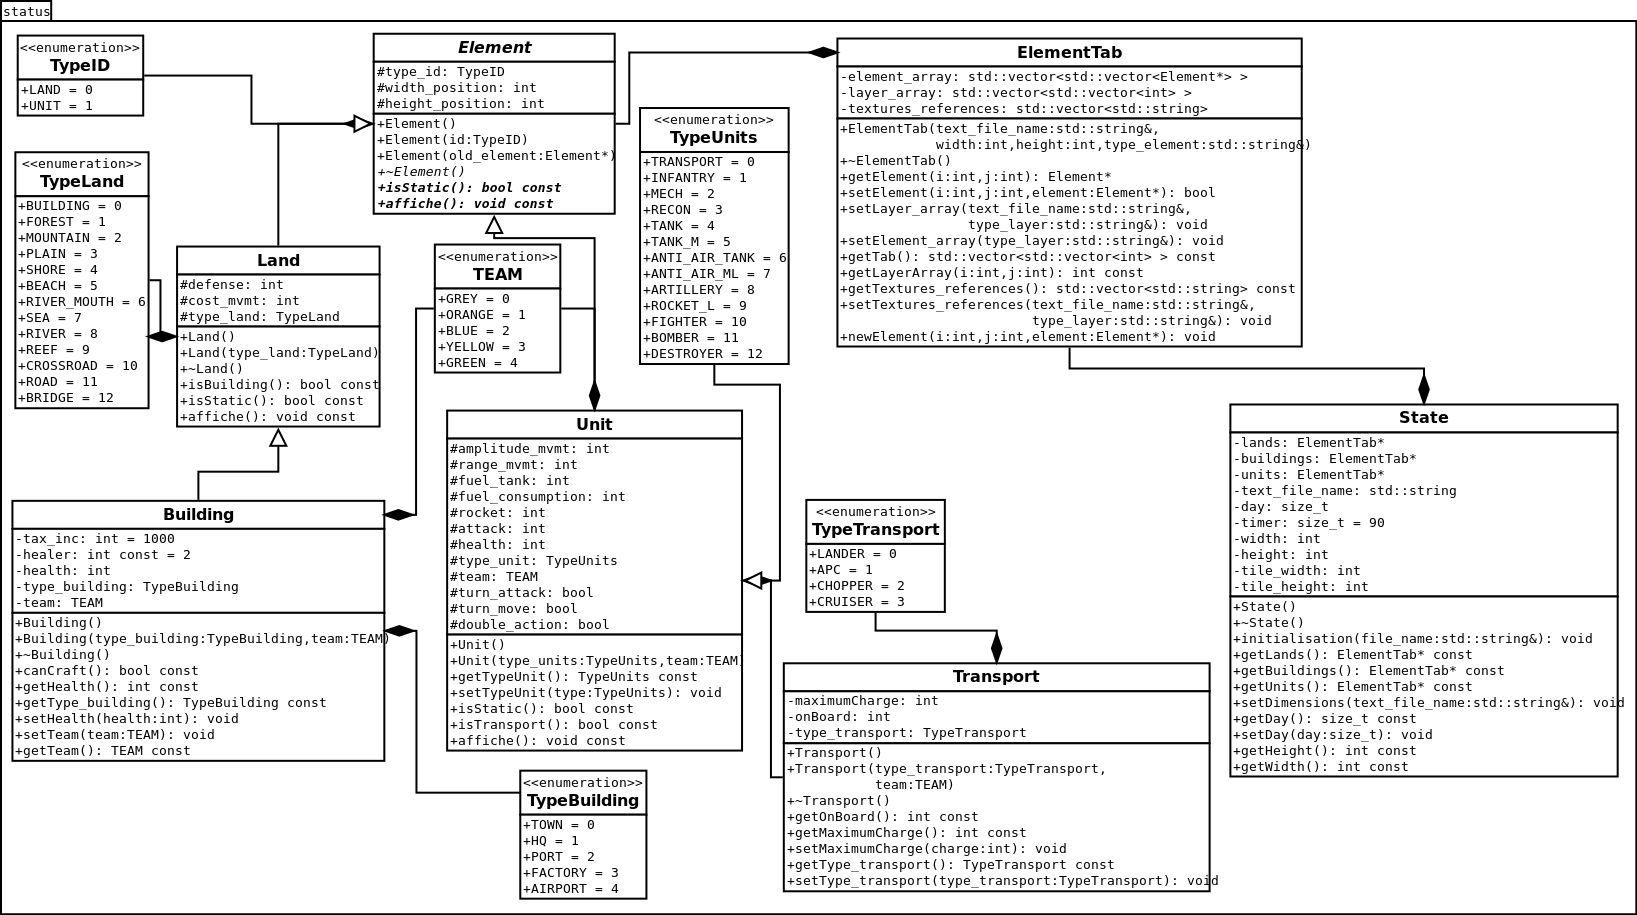
\includegraphics[scale=0.43]{Status.png}
    \caption{Diagramme des classes d'état}
\end{figure}
\end{landscape}
    
\newpage

\chapter{Rendu : Stratégie et Conception}
    \section{Stratégie de rendu d'un état}
    \paragraph{}La stratégie que nous avons établi pour le rendu d'un état est une stratégie de bas niveau. Nos scènes sont coupées en plans : un plan pour le niveau qui contient différents paysages (plaine, montagne, forêt,etc.), un plan d'unités mobiles (infanterie, tank, navire,etc.), et un plan d'informations d'état du jeu (vie, jauge de pouvoir,etc.).. Chaque plan possède différentes informations : une unique texture contenant les tuiles, une unique matrice avec la position des éléments, un tableau de nos plans, le nom du fichier texte à partir du quel nous générons notre état, un tableau des différentes textures, les dimension de la fenêtre ainsi que les dimensions de tuiles. 
    
    \paragraphe{}L'organisation du rendu se fait à partir de l'état et de la détection d'un changement. Si le changement dans l’état donne lieu à un changement permanent dans le rendu, on met à jour le morceau de la matrice du plan correspondant. Pour les changements non permanent, comme les éléments mobiles, nous tiendrons à jour une liste d’éléments visuels à mettre à jour (=> modification de la matrice du plan) automatiquement à chaque rendu d’une nouvelle frame.  
    
   % \paragraphe{Synchronisation}
    
    \section{Conception logiciel}
    \paragraph{} Le diagramme du rendu est présent en Figure 3.1.
    
    \paragraphe{}\textbf{Plans:} Le principal objectif des instances de Layer est de donner les informations basiques pour former les éléments bas-niveau à transmettre à la carte graphique; ces informations sont données à une instance de Surface, et la définition des tuiles est contenu dans une instance de TileSet. 
    % définir se que font StateLayer et ElementTabLayer
    
    \paragraphe{}La méthode setSurface() fabrique une nouvelle surface à partir de notre fichier texte, grâce aux informations contenues dans ce fichier on peut lui demander d'initialiser la liste des tableaux de vertex. Pour afficher le niveau, elle demande les dimensions de la fenêtre avec initQuads().Puis, pour chaque cellule du niveau, elle fixe leur position avec setQuadPosition() et leur tuile avec setQuadTextureCoordinates(). 
    
    \paragraphe{}\textbf{Surfaces:} Chaque surface contient une texture du plan et une liste de paires de quadruplets de vecteurs 2D. Les éléments texCoords de chaque quadruplet contient les coordonnées des quatre coins de la tuile à sélectionner dans la texture. Les éléments position de chaque quadruplet contient les coordonnées des quatre coins du carré où doit être dessiné la tuile à l’écran. 
    
    \paragraphe{}\textbf{Tuiles:} La classe TileSet contient un tableau de toutes les tuiles d’un même plan. Elle peut grâce à la méthode getTile(), récupérer la tuile correspondant à un indice de son tableau, et à partir de cette tuile on peut savoir ses dimensions ainsi que l'emplacement de sa texture dans nos dossiers. Pour obtenir ces informations, un client dispose des méthodes getWidth(), getHeight() et getAdressFile(). 

    
    \newpage
\thispagestyle{empty}
\begin{landscape}
\begin{figure}[h]
\begin{center}
    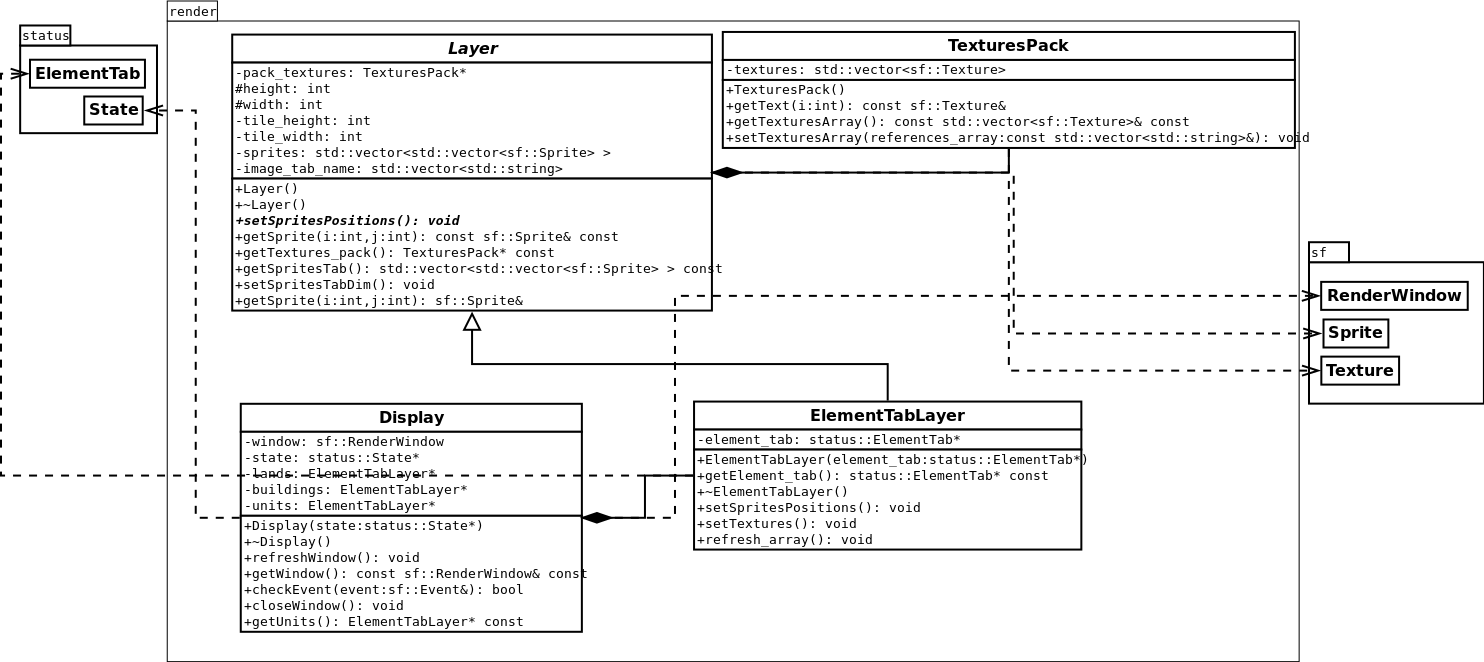
\includegraphics[scale=0.48]{render.png}
    \end{center}
    \caption{Diagramme du rendu}
\end{figure}
\end{landscape}
    
\newpage

\chapter{Règles de changement d'état et moteur du jeu}
\section{Tours et horloges}
\paragraph{}Lors du tour d'un joueur, plusieurs actions peuvent être effectuées (il est tout à fait possible de passer sont tour). Une action entraîne un changement d'état. Un changement d'état est instantané mais l'animation d'un déplacement ou d'une attaque introduit un temps de pause pendant lequel le joueur ne peut pas effectuer une autre action. Afin de ne pas bloquer la partie, un temps total par tour doit être imposé. Le jeu introduira donc deux horloges : une pour le décompte du temps de tour, une autre pour afficher un changement d'état qui a déjà été effectué.

\section{Changement extérieurs}
\paragraph{}Ce sont les changements demandés par une entrée externe (pression de touche ou réseau).
Les différents changements extérieurs peuvent être un chargement de carte, une attaque, un déplacement, la création d'une nouvelle unité, la capture d'un bâtiment, la fusion de deux unités ou encore la fin d'un tour.

\section{Changements autonomes}
\paragraph{}Les différents changements autonomes qui peuvent avoir lieux sont :
\begin{itemize}
    \item la capture d'un bâtiment fait diminuer le nombre de points de capture restant avant qu'il soit acquis
    \item l'attaque d'une unité par une autre fait diminuer les points de vie de l'unité attaquée et les munitions de l'unité attaquante si les munitions sont spécifiques
    \item le déplacement d'une unité fait diminuer ses points de carburant/rations en plus de ceux obligatoires à chaque tour
    \item la fusion d'une unité avec une autre identique fait disparaître l'une des deux, additionne les points de vie et crée une rentrée d'argent si la somme des points de vie dépasse la limite maximale
    \item un changement de tour crée une rentrée d'argent proportionnelle au nombre de villes possédées
\end{itemize}

\section{Conception logiciel}
\paragraph{}Le diagramme des classes pour le moteur du jeu est présenté en Figure  4.1. Le moteur se compose de différentes classes(Command et Action) qui permettent la mise en oeuvre différée de commandes extérieures sur l'état du jeu.
\paragraph{}\textbf{Classes Command:} Le rôle de ces classes est de représenter une commande, quelque soit sa source. Pour chacune de ces classes, on a défini un type de commande avec CommandTypeId pour pouvoir identifier la classe d'une instance.
\begin{itemize}
    \item \emph{LoadMap} : Charge un niveau depuis un fichier;
    \item \emph{CreateUnit} : Crée une unité;
    \item \emph{MoveUnit} : Déplace une unité;
    \item \emph{AttackUnit} : Une unité attaque une unité adverse;
    \item \emph{CaptureBuilding} : Une unité capture un bâtiment ( neutre ou adverse);
    \item \emph{ResetUnits} : Détruit les unités sur le terrain;
    
\paragraph{}\textbf{Classes Action:}  Chaque commande, lorsqu’elle est exécutée, donne lieu à certain nombre d’actions à réaliser, suivant les cas. Ces actions sont concrétisés par les classes filles de Action. Cela permet d’atomiser les opérations effectives, et donc de les inverser grâce à l’appel aux methodes undo(). Ces classes nous permettent donc d’annuler les conséquences de commandes, et nous servent à remonter dans l’arbre des états pour l’intelligence artificielle avancée (algorithme minmax). 

\paragraph{}\textbf{Engine:} Cette classe correspond au moteur du jeu. Elle stocke les commandes dans une std : :map avec clé entière. Ce mode de stockage permet d’introduire une notion de priorité : on traite les commandes dans l’ordre de leur clés, de la plus petite à la plus grande. Lorsqu’une nouvelle époque démarre, c'est à dire quand on appelle la méthode update(), le moteur appelle la méthode execute() de chaque commande, incrémente l’époque, puis supprime toutes les commandes. Il en résulte une pile d’actions qui, si on les appliquent en ordre inverse, permettent d’annuler les commande précédemment invoquées.


    \newpage
\thispagestyle{empty}
\begin{landscape}
\begin{figure}[h]
    \begin{center}
    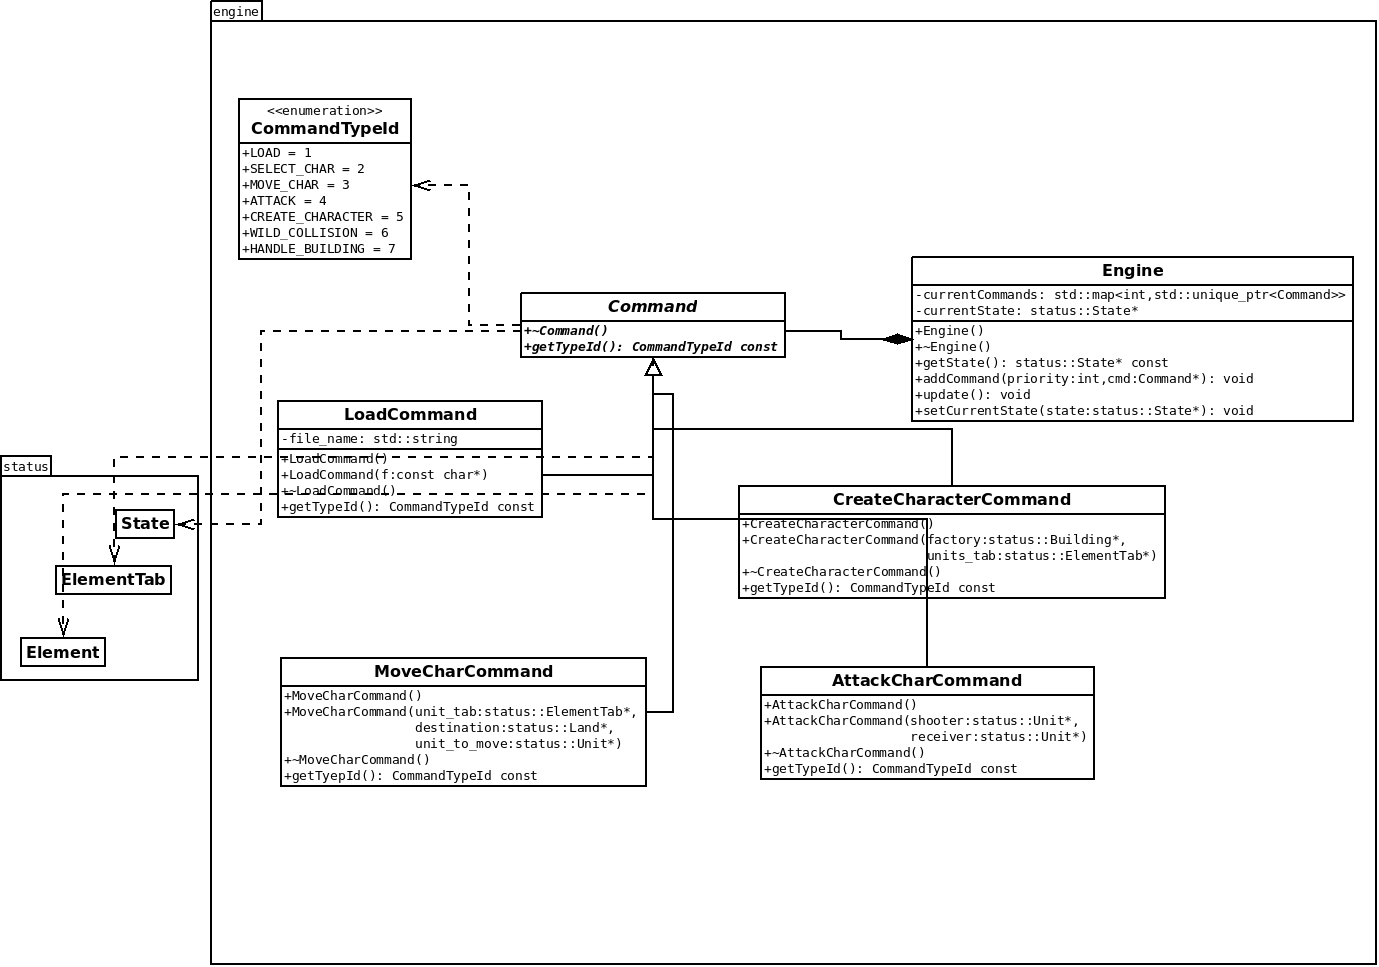
\includegraphics[scale=0.35]{engine.png}    
    \end{center}
    \caption{Diagramme de l'engine}
\end{figure}
\end{landscape}

\chapter{Intelligence Artificielle}
\section{Stratégie}
\subsection{Intelligence artificielle bas-niveau}
\paragraph{}Le principe consiste à donner une liste de commandes possibles aux unités et de parcourir le tableau des unités afin qu'elles effectuent une action choisie aléatoirement dans la liste de commandes passées en argument. Pour respecter le concept de carte vide au premier tour, un passage dans le tableau des bâtiments sera effectué afin de générer des unités (aléatoirement si possible) et ensuite de parcourir le tableau des unités créées pour effectuer des commandes aléatoires.
\subsection{Intelligence basée sur des heuristiques}
\paragraph{}Pour obtenir un comportement meilleur que le hasard, nous voulons permettre à l'IA de rechercher l'ennemi le plus proche pour l'attaquer ou de chercher le bâtiment le plus proche pour le capturer ou soigner l'unité en déplacement.Pour cela nous allons fabriquer des cartes de distances.
Pour calculer ces cartes, nous utilisons l’algorithme de Dijkstra.
\subsection{Intelligence avancée}
\paragraphe{}Nous proposons une intelligence plus avancée en suivant les méthodes de résolution de problèmes à états finis. Dans cette configuration, un état est un état du jeu à une époque donnée, tel que défini dans la section état. Les arcs entre les sommets du graphe d’état sont les changements d’états.. Passer d’un sommet du graphe d’état à un autre reviens à passer d’une époque à une autre du jeu, fonction de l’ensemble des commandes reçues (clavier, réseau, IA,...). L’évaluation/score d’un sommet/état du jeu n'a pas encore pu être déterminée.

\paragraphe{}Pour que notre AI prenne les meilleures décisions, nous suivons des méthodes basées sur les arbres de recherche, avec une propriété importante. En effet, nous n’envisageons pas de dupliquer l’état du jeu à chaque sommet du graphe d’état. Nous n’allons considérer qu’un seul état que nous modifions suivant la direction choisie par la recherche. Si le sommet suivant est à une époque suivante, i.e. on descend dans l’arbre de recherche, on applique les commandes associées, et notre état gagne une époque. Si le sommet suivant est à une époque précédente, i.e. on remonte dans l’arbre de recherche, on annule les commandes associées, et notre état retrouve sa forme passée. Ces pour cela que plus tôt nous créons les classes Action.

    \newpage
\section{Conception logiciel}
\paragraphe{}Le diagramme des classes pour l’intelligence artificielle est présenté en Figure 5.1.
\paragraphe{}\textbf{Classes AI:}Les classes filles de la classe AI implante différentes stratégies d’IA :
\begin{itemize}
    \item RandomAI : Intelligence aléatoire
    \item HeuristicAI : Intelligence heuristique
     \item DeepAI : Intelligence avancée
\end{itemize}
\paragraphe{}\textbf{PathMap:}La classe PathMap permet de calculer une carte des distances à plusieurs unités. Pour chaque case « espace » du niveau, on peut demander un poids qui représente la distance à ces objectifs. Pour s’approcher d’un objectif lorsqu’on est sur une case, il suffit de choisir la case
adjacente qui a un plus petit poids. Deux cartes de distantes
sont crées en début de tour :
\begin{itemize}
    \item adv\_units\_map : Objectif cases unités adverses, pour pouvoir attaquer l'unité la plus proche
    \item building\_map : Objectif building, pour s’emparer des building ennemis ou se soigner si le building nous appartient
\end{itemize}

\paragraphe{}\textbf{DeepAI:} Nous proposons ici une implantation pour une IA basée sur la résolution de problèmes à état fini, tel que défini dans la section précédente. L’algorithme utilisé est une version du minimax pour deux joueurs. 
\newline (Le critère d'évaluation n'a pas encore été trouvé, car nous voulons évaluer l'avancée d'un joueur sur la distance de ces unités au QG adverse (car le but est de le capturer) mais aussi au nombre d'unité encore présentes sur le terrain ainsi que le nombre de bâtiments possédés, car ce sont des avantages déterminants pour la réussite du joueur).
\end{itemize}

    \newpage
\thispagestyle{empty}
\begin{landscape}
\begin{figure}[h]
    \begin{center}
    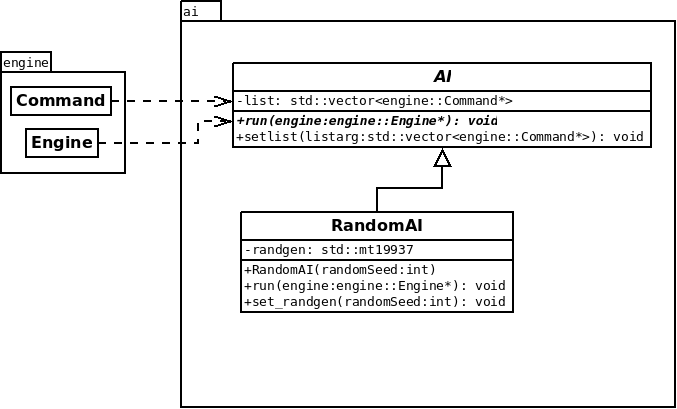
\includegraphics[scale=0.45]{ai.png}
    \end{center}
    \caption{Diagramme de l'intelligence artificielle bas-niveau}
\end{figure}
\end{landscape}
\end{document}

